\chapter{Basic Biochemistry} \label{ch:bio}

\section{{\em E. coli}: The Model Procaryote}

% What it is
Synthetic biologists work with a variety of organisms. The choice of
which organism depends on the application in mind and also on the
innate abilities of the organism. For example, if the goal is to
produce butanol from sunlight, an organism that photosynthesizes and
that normally produces some useful immediate precursor to butanol is
an appropriate starting point (for example, the {\em
  cyanobacteria}). If the goal is to develop a medical treatment, a
simple eukaryote (such as the yeast {\em S. cerevisiae}) would be
appropriate. For our purposes, which are to design and debug basic,
portable biochemical circuits and regulatory processes, the ideal
organism is the humble bacterium {\em Escherichia coli}, or {\em
  E. coli} -- shown in Figure~\ref{fig:ecoli}. 

\begin{figure}
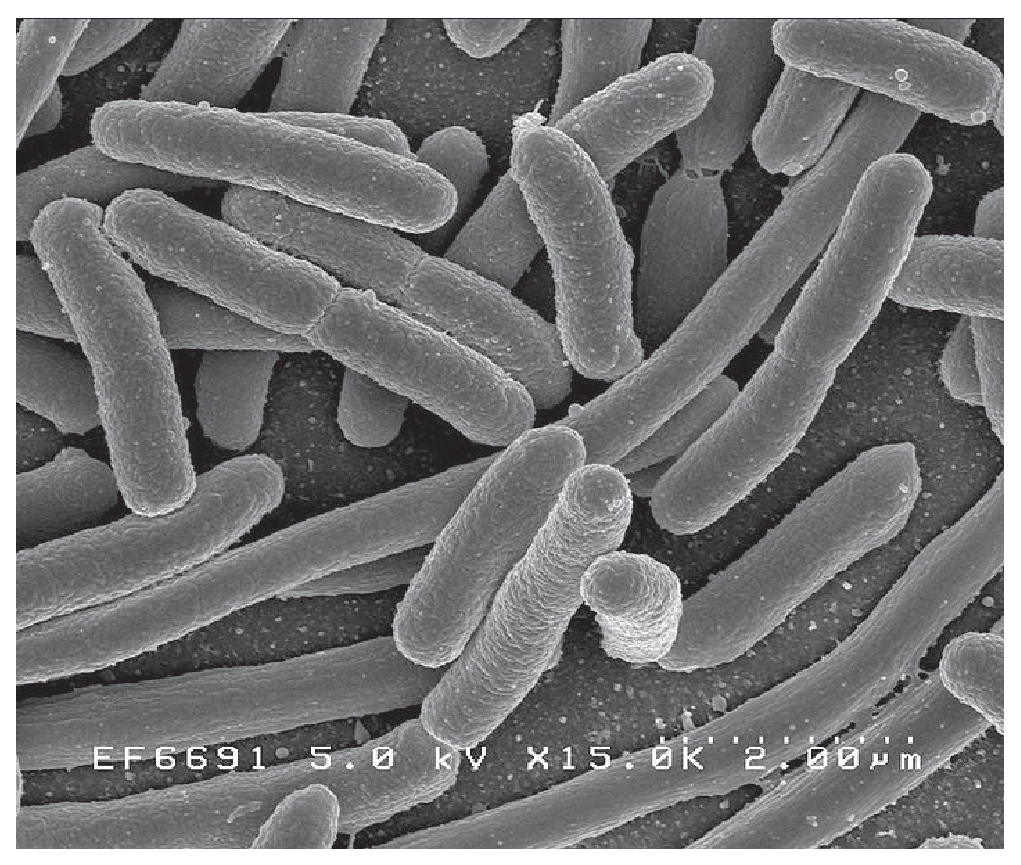
\epsfig{file=figures/ecoli.eps, scale=0.6}
\caption{\label{fig:ecoli} A scanning electron micrograph image of
  {\em E. coli} cells. Each cell is approximately 2 $\mu$m long and
  has a volume of about 1 $\mu\mathrm{m}^3$. Several of the cells in
  this image have just divided end-to-end, producing genetically
  identical daughter cells. Credit: Rocky Mountain Laboratories,
  NIAID, NIH. }
\end{figure}

{\em E. coli} is very well studied. Many of the most important genetic
and molecular processes in biology were first discovered in {\em
  E. coli}, and at least eight Nobel prizes are associated with
discoveries made with it (e.g. Monod, Lederberg, Taum and Beadle,
...). {\em E. coli} is, furthermore, the workhorse in almost every lab
that uses DNA: It is used basically as a DNA factory -- happily
replicating any DNA you put into it. {\em E. coli} are used in
industry as well. For example, the production of insulin, which used
to be obtained from pig pancreases, is now done in genetically
modified {\em E. coli} \cite{insulin}. Because {\em E. coli} is so
well understood, if {\em you} want to know how something in {\em
  E. coli works} so that you can hack it, you will more often than not
be able to find someone to help you. In contrast, if you work on an
obscure microorganism, and you will most likely be on your own.

{\em E. coli} is found naturally in the human gut, along with numerous
other kinds of bacteria. Humans can't live without their bacteria,
which help them digest their food, among other responsibilities. Most
of the cells on and in your person, in fact, are (very small) bacteria
cells and not (big) human cells. The strains of {\em E. coli} used in
the lab are all descendants of {\em E coli} K-12, which was isolated
at Stanford University 1922 from human feces. It was kept there for
years as a stock strain and has, in fact, evolved to live alone in the
comfort of the lab. Due to their relaxed lifestyle, K-12 can barely
survive outside of the lab and is generally considered to be harmless
(unlike the strains of {\em E. coli} that sometimes infect foodstocks
\cite{taco-bell}). You can now obtain from a variety of sources a huge
range of strains related to K-12, each with its own ``features''. Some
strains produce lactose digesting enzymes, some can conjugate with each
other, some have had their DNA repair genes knocked out, and so on
\cite{cgsc}.

To some extent, if a synthetic biologist can get a device to work in
{\em E. coli}, the principles of how its works should apply to other
organisms as well and often the circuit can be transplanted as is into
other organisms. As Jaques Monod said, ``All that is true for the {\em
  Colon bacillus} [e.g. {\em E. coli}] is true for the elephant''
\cite{monod}. Monod's observation is that all life forms on earth use
essentially the same architecture -- of which this chapter is an
overview.

In particular, this chapter describes, at a very high level, the
architecture of organisms like {\em E. coli} -- that is {\em
  procaryotes} (cells not having a nucleus). The goal is to ground the
ideas that appear later in the book in systems inside a
well-understood model organism. Note that this chapter is not even
remotely a good substitute for a textbook on biochemistry
\cite{nelson-cox}, a textbook on cell biology \cite{thecell}, or a
text book on bacterial genetics \cite{bact-genetics}.

\section{Molecules in the Cell}

Bacteria, including {\em E. coli}, are single celled {\em procaryotic}
organisms. Among other things, this means that they do not have a
nucleus containing their genomic DNA, and they do not have
particularly sophisticated ways of processing their RNAs and
proteins. Rather, the DNA and most of the other molecules that make up
an {\em E. coli} cell's machinery, are located in the main interior of
the cell called the {\em cytoplasm} or they are part of the cell {\em
  membrane} enclosing the cytoplasm. In this section we describe at a
high level what most of the important molecules are called and what
they do in the cell. It is difficult to know where to start with such
a description as each type of molecular interacts with other types so
that in describing RNA, we need to talk about DNA and proteins, for
example. The order of presentation below is therefore somewhat
arbitrary. The reader might consider reading this section twice to
resolve references to one type of molecule while introducing another
type of molecule.

% Molecules (DNA, RNA, Protein, small molecules, etc) 

\paragraph{DNA} Perhaps the most important kind of molecule in the
cell is {\em deoxyribonucleic acid} or DNA. A big DNA molecule, called
the genomic DNA, stores almost all of the information required to
build and run an {\em E. coli}. DNA molecules are long, oriented
polymers (long chains) of four different types of {\em nucleotides},
as seen in Figure~\ref{fig:dna}. Each nucleotide consists of a {\em
  base}, adenine (or A), thymine (or T), guanine (or G) and cytosine
(or T), attached to a deoxyribose sugar, and a phosphate group. The
nucleotides in a DNA molecule are strung end to end to form a long
chain or, more often, a circle. Since the nucleotides in a DNA molecule
can appear repeatedly and in any order, there are in fact $4^N$
different DNA molecules of length $N$. For a standard strain of {\em
  E. coli}, $N \approx 4.6$ million. If we were to randomly
make DNA molecules of this length and try to ``boot them up'' inside a
cell, the chance we'd accidentally make a working organism like {\em
  E. coli} is approximately one in $4^{10^6}$. Apparently, we need to
understand how to put together (or program) DNA molecules more
systematically.

\begin{figure}
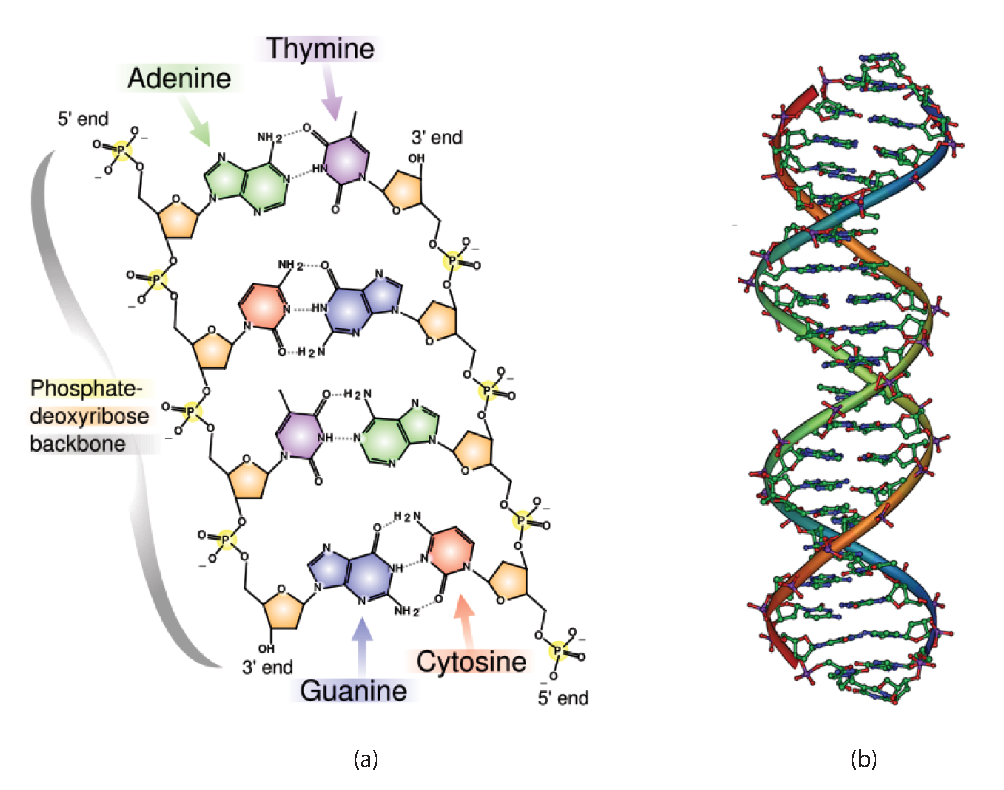
\epsfig{file=figures/dna.eps, scale=0.75}
\caption{\label{fig:dna}The structure of DNA. (a) Bases and base
  pairing. DNA consists of polymers of bases of four different types:
  adenine (or A), thymine (or T), guanine (or G) and cytosine (or T)
  each attached to a deoxyribose sugar. Two stands of DNA will form a
  duplex if they are complimentary: A sticks to T and C sticks to
  G. Note also that DNA has an orientation: the 5' end is different
  than the 3' end. (b) The double-helix. Double stranded DNA folds
  into a double-helix the 3D structure of which can form highly
  specific binding sites for regulator proteins.}
\end{figure}

DNA molecules are typically not found alone. Instead each DNA strand
is attached, with {\em hydrogen bonds}, to a {\em
  complimentary strand} via {\em Watson-Crick} base pairing. It turns
out that A sticks to T and C sticks to G, so the strand $5'-ATAGCA-3'$
is complimentary to $3'-TATCGT-5'$. In this notation, the strands are
oriented from the $5'$ to the $3'$ ends (see Figure~\ref{fig:dna}). It
is this complimentary nature of DNA that makes it ideal for
representing and copying information. If you (or the cell) unzips a
double stranded piece of DNA, each makes a template for the
construction of a new complimentary strand. This copying occurs every
time a cell divides with incredible accuracy: the error rates are
about one mismatch in every $10^9$ bases copied \cite{dna-error-rate}.

In later sections of this chapter, we describe at a high level how 
DNA is interpreted by the machinery in the cell to direct growth,
program how the cell responds to its environment, and so on.

\paragraph{RNA} Although we just said that DNA is the most
important molecule in the cell, it is hard to overstate the importance
of {\em ribonucleic acid} or RNA. RNA is structurally similar to DNA
except that the bases are attached to a ribose sugar instead of a
deoxyribose sugar and instead of thymine RNA contains uracil. The
similarity ends there however. While DNA is a stable information
carrier, RNA is less stable and to some extent defines the changing
internal state of a cell. Furthermore, RNA is generally found single
stranded, often modified by the addition of other small molecules, and
is typically folded up on itself more like a protein, as shown in
Figure~\ref{fig:rna}. Finally, while DNA is a massive circular
double-stranded beast, RNAs are typically short (from 10 to 3000 bases
long).

\begin{figure}
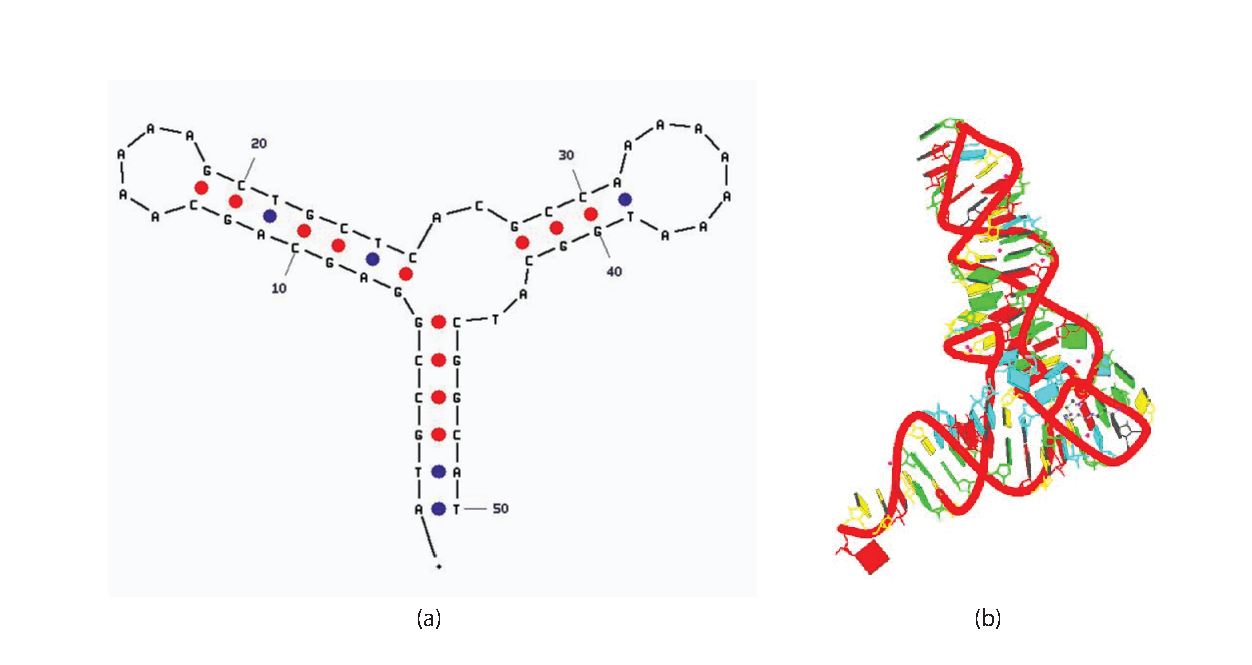
\epsfig{file=figures/rna.eps, scale=0.6}
\caption{\label{fig:rna} RNA. (a) The topology of a typical RNA
  molecule. The RNA strand folds up on itself in predictable ways with
  A sticking to U and C sticking to G. (b) The 3D structure of a
  transfer RNA.}
\end{figure}

All RNAs in the cell are {\em transcribed} (see below) from regions of
the genome called genes. Once transcribed, an RNA is destined for one
of a surprisingly many roles in the cell. {\em Messenger RNA} or mRNA
is an intermediate representation of a protein. Its role is to carry
the information for how to build a protein from the genome to the
protein building machinery. The protein-building machinery itself is
built primarily from two types of RNA called {\em transfer RNA} or
tRNA and {\em ribosomal RNA} or rRNA. tRNAs are the interface between
triples of bases called codons (found on on mRNAs) and the amino acids
corresponding to the codons. Ribosomal RNAs glob together into
molecular machines called ribosomes that translate mRNAs into proteins
using tRNAs (this process is described below). Finally, there
regulatory RNAs of many type. For example, {\em small interfering
  RNAs} or siRNAs are bits of RNA that are complimentary to regions of
mRNAs that prevent their translation into protein. Another type of
regulator RNA are the various {\em ribozymes}, which are RNAs that
exhibit catalytic activity, for example, cleaving other RNAs in
specific (and programmable) regions.

\paragraph{Protein} Proteins are folded up polymers consisting of
chains of sub-units called {\em amino acids}. There are 20 different
amino acids (see Figure~\ref{fig:genetic-code}) that are found in
normal living systems. Amino acids all have the same basic form
consisting of an amino group ($H_3N$) and a carboxyl group ($CO_2H$)
on either side of a $H-C-R$ group. The $R$ is another group called the
{\em residue} that determines the type of amino acid. Each amino acid
is different: it may be hydrophobic or hydophyllic; it may be polar or
not; etc. 

Amino acids can form chains due to their modular nature. The amino
group of one can stick to the carboxyl group of another forming a
peptide bond and releasing a water molecule, as shown in
Figure~\ref{fig:peptide-bond}. By continuing this process, any chain
of up to thousands of amino acids can be formed. Due to the different
chemical natures of the amino acids, the chain will {\em fold up} into
different shapes. The resulting protein will have pockets and grooves
and bumps each with a function determined by the amino acids near that
feature. Thus, proteins are programmed blobs of matter with programmed
chemical functionality -- and the possible functionality seems to be
limitless. Almost every important function inside a cell is performed
in part by a protein. They regulate the expression of genes; help
transport molecules in and out of the cell; a particular protein {\em
  enzyme} can very specifically increase the activity of a particular
chemical reaction; some proteins polymerize into long, rigid chains
that give cells structure; protein motors can pull cargo around inside
cells; some proteins are hormones that carry signals to other cells;
and on and on. This programmability of function is unparalleled.

\begin{figure}
\centering
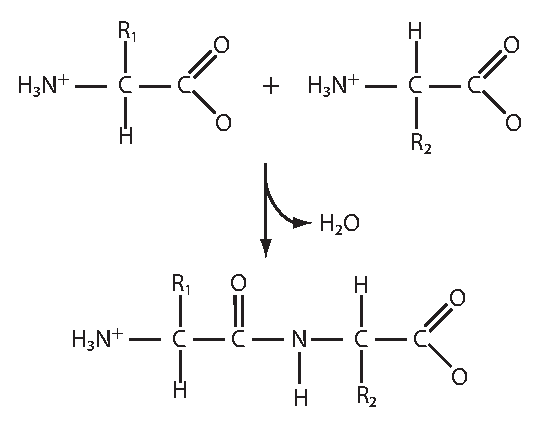
\epsfig{file=figures/peptide-bond.eps, scale=0.8}
\caption{Two amino acids condense to form a peptide bond. Long chains
  of amino acids fold up to form proteins. The amino group of the
  chain is called the N-terminus and the carboxyl group is called the
  C-terminus. \label{fig:peptide-bond}}
\end{figure}

An example protein is GFP, discussed in the introduction. It consists
of a sequence 264 amino acids with a mass\footnotemark of just over 27
kDa. This sequence of amino acids, shown in Figure~\ref{fig:gfp}(a),
folds up into a secondary structure due to the natural attractions and
repulsions of its constituent amino acids, as shown in
Figure~\ref{fig:gfp}(b). Stretches of a protein often form into
recognizable substructures, either $\alpha$-helices or
$\beta$-sheets. The former are helical regions and the latter are
regions that interact with other $\beta$ regions to form sheet like
structures. Figure~\ref{fig:gpf}(c) shows a cartoon of GFP in which helix
and sheet structures are highlighted. Sub-structures that are neither
sheets nor helices are called random coils and are shown as simple
lines are ropes. 

\footnotetext{Masses of molecules are often measured in Daltons
  (Da). One Dalton is approximately the mass of one Hydrogen atom.}

\begin{figure}
\centering
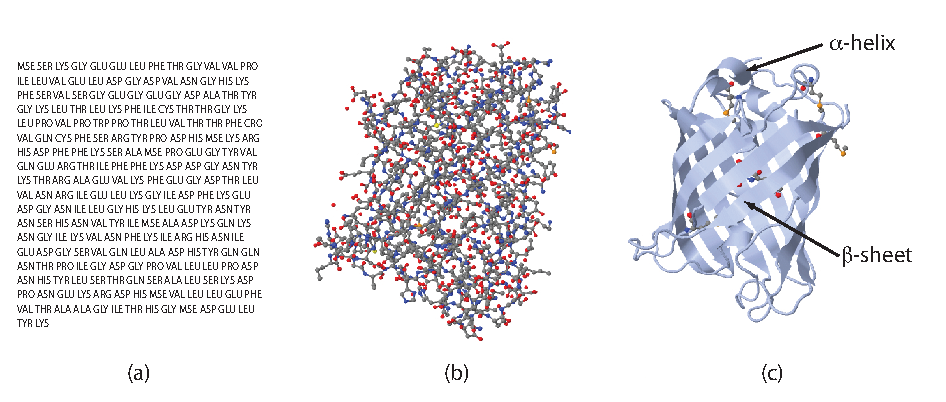
\epsfig{file=figures/protein.eps, scale=0.8}
\caption{The structure of green fluorescent protein (GFP), downloaded
  from the protein data bank. (a) The sequence of residues. Each
  three letter code corresponds to a different residue, according to
  the scheme in Figure~\ref{fig:genetic-code}. (b) The three
  dimensional or secondary structure of GFP. The relative coordinates
  of each residue are typically determined empirically using X-Ray
  crystallography. (c) The cartoon version of the protein showing more
  clearly its structure as a barrel-shaped molecule. \label{fig:gfp} }\end{figure}

\paragraph{Small Molecules} The are an enormous variety of small
molecules in the cell (besides, of course, $H_2O$) that the cell is
very adept at processing. Simple sugars, carbohydrates, lipids,
alcohols, amino acids, nucleotides, signaling molecules and
antibiotics are just some of the substances that cells know how to
make. These molecules are of great interest to metabolic engineers who
see cells as programmable chemical processing plants. By changing the
expression of protein enzymes or by adding the genes for new protein
enzymes into an organism, new substances can be made by old organisms. 


\section{Processes}

\subsection{Transcription}

% Processes: Transcription, translation

The long chain of genomic DNA inside a cell is dived up into segments
called {\em genes}. These genes take on many forms. The most basic
form consists of a short sequence of DNA called a {\em promoter},
after which follows a long sequence (up to thousands of base pairs) of
DNA called a {\em template} containing the information represented by
the gene, and terminated by a short sequence called a {\em
  terminator}. See Figure~\ref{fig:transcription}(a).

\begin{figure}
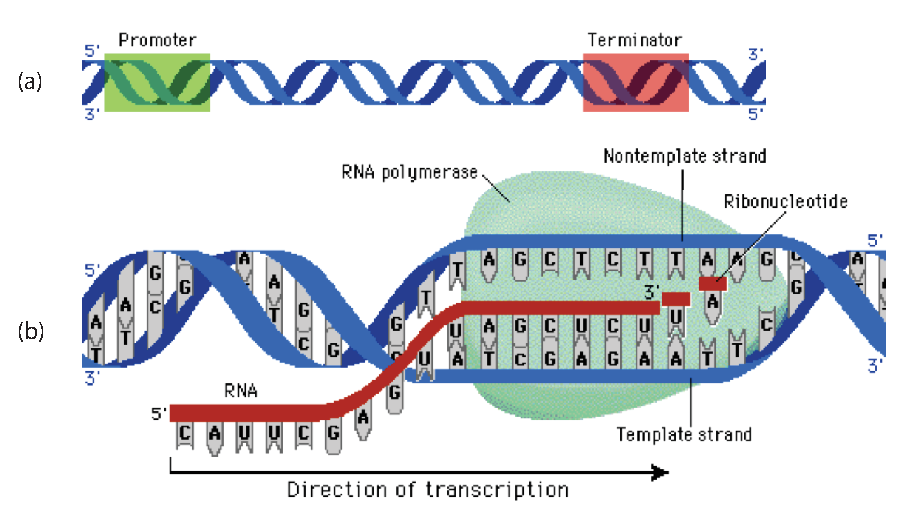
\epsfig{file=figures/transcription.eps,scale=0.75}
  \caption{\label{fig:transcription} (a) A simple gene containing a
    promoter, a template, and a terminator region. (b) The process by
    which RNA polymerase (RNAP) transcribes the template DNA into an
    RNA transcript. }
\end{figure}

The promoter region of a gene has a specific three-dimensional
structure due to the sequence of nucleotides in the region. This
structure allows an important enzyme called {\em RNA Polymerase}
(RNAP) to specifically bind to the promoter region (RNAP is actually a
collection of proteins that act together as an enzyme). Once there,
RNAP locally splits the DNA double helix in the template region and
builds an RNA molecule complimentary to the template. The new piece of
RNA is called the {\em transcript} from the template. In bacteria,
this happens at an astounding rate of about 80 nucleotides per second
\cite{alon-book}. The RNAP continues transcription of the template
until it reaches the terminator, at which point the RNAP falls of the
gene. See Figure~\ref{fig:transcription}(b).

A gene that is ``on'' (see regulation, below) may have many RNAP
enzymes actively transcribing the gene at any given time and so there
may be many transcripts from the gene present in the cell at any given
time. Also, RNA is degraded fairly quickly. The signals and conditions
represented by RNAs are therefore temporary.

The RNA transcripts in the cell have many possible destinies,
summarized below:

\smallskip

\begin{tabular}{lll}
Messenger RNA (mRNA) & \ & mRNA can be {\em translated} into one or \\
                     & \ & several proteins (see Translation, below).  \\
Transfer RNA (tRNA)  & \ & tRNA is the interface between mRNA and protein.  \\
                     & \ & Each type of tRNA is modified to carry a \\
                     & \ & specific amino acid on one end and has an \\
                     & \ & {\em anticodon} on the other end \\ 
Ribosomal RNA (rRNA) & \ & The ribosome is a complex machine consisting \\
                     & \ & of RNA and protein that translates mRNA into \\
                     & \ & protein by stringing together amino acids \\
                     & \ & presented by tRNAs \\
Other                & \ & Other RNAs can fold into RNA enzymes called \\
                     & \ & ribozymes or (esp. in Eucaryotes) form small \\
                     & \ & antisense RNA or micro RNA      
\end{tabular}

\subsection{Translation}

Some of the RNA transcribed has a chance to be {\em translated} into
protein, as long as it doesn't get degraded first or isn't blocked by
some antisense RNA. An mRNA contains a {\em ribosomal binding site} or
RBS to which the enzyme responsible for translation, the {\em ribosome}
binds. Once bound, the ribosome moves forward (in the 5' to 3'
direction) on the mRNA until it encounters the sequence AUG -- the
{\em start codon} and also the codon for Methionine. 

\begin{figure}
\centering
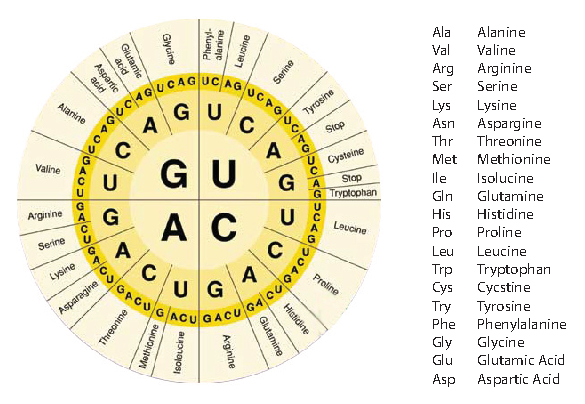
\epsfig{file=figures/genetic-code.eps}
\caption{\label{fig:genetic-code}
(a) The genetic code. The first letter in a codon is at the center. (b) Abbreviations. 
}
\end{figure}

There are other three letter codons as well, after the start
codon. Each codon corresponds to a specific amino acid according to the
{\em genetic code} shown in Figure~\ref{fig:genetic-code}. This code
is almost exactly the same in every organism ever studied -- which is
why a gene from one organism is likely to work when inserted into
another organism. The ribosome steps through each codon starting with
the start codon until it reaches a {\em stop codon}. 

\begin{figure}
\centering
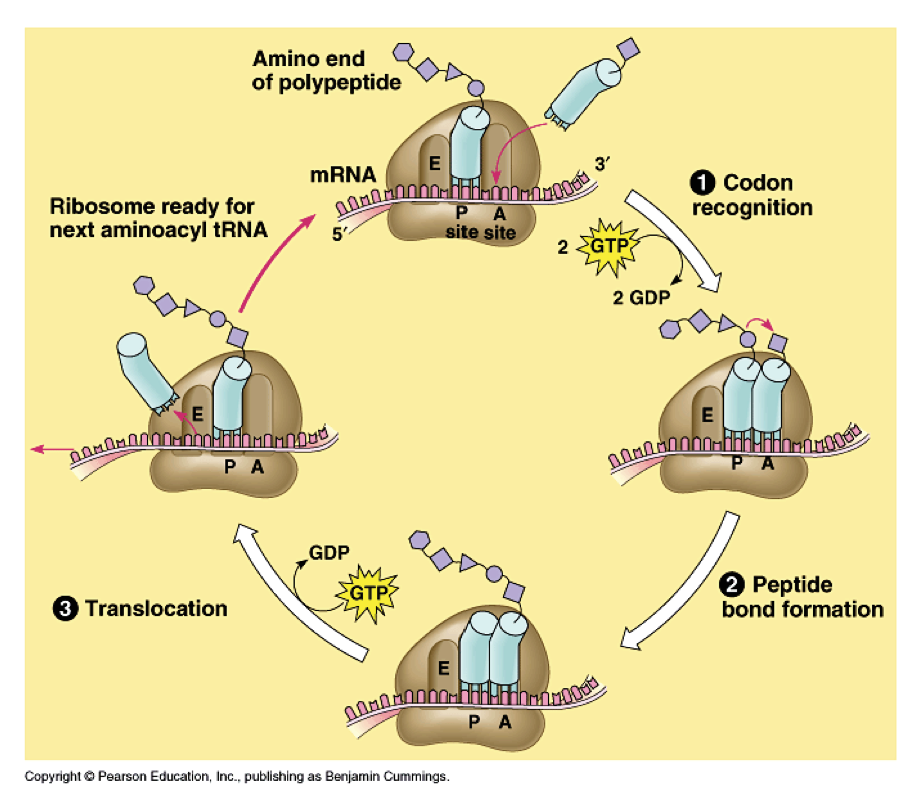
\epsfig{file=figures/translation.eps, scale=0.75}
\caption{\label{fig:translation} The process of translation. The
  Ribozyme binds onto the {\em ribosomal binding site} of an mRNA,
  moves forward to the start codon, and thne translates the codons in the
  mRNA into protein, ending at a stop codon.}
\end{figure}

Specifically, when a ribosome parks at a codon, a tRNA having the
complimentary sequence, the anti-codon, docs at the codon, held in
place by the ribosome. Next, the amino acid at the other end of the
tRNA is attached to a growing chain of amino acids by the
ribosome. Then the ribosome steps forward to the next codon and
discards the transfer RNA (without the amino acid). This process
continues until the stop codon is reached at which point the sequence
of codons in the mRNA has been completely translated into a sequence
of amino acids. The amino acid chain folds up into a functional
protein while it is being translated or very soon after translation ends. 

The ribosome, which consists of several subunits of both rRNA and
protein is arguably the most remarkable molecular machine in the
natural world. Not only are they responsible for translation and
protein biosynthesis, they do their job very well -- correcting for
errors and processing 12 to 21 amino acids {\em per second}. 


In should be noted that transcription and translation, in procaryotes
anyway, occur simultaneously. A given gene may have several RNAP
molecules transcribing mRNAs off of it at any given time. Each of the
mRNAs may have several ribosomes attached to it, translating protein.

\subsection{Regulation}

% constitutive vs regulated
Some genes are on all the time, meaning that RNA transcripts are
constantly generated by RNAP using the template in the gene. Such
genes are called {\em constitutively expressed}. Most genes, however,
are regulated in some way so that the RNA transcripts for the gene are
only generated when they are needed. The most common way for a gene to
be regulated is via proteins called {\em transcription factors}.

\begin{figure}
\centering
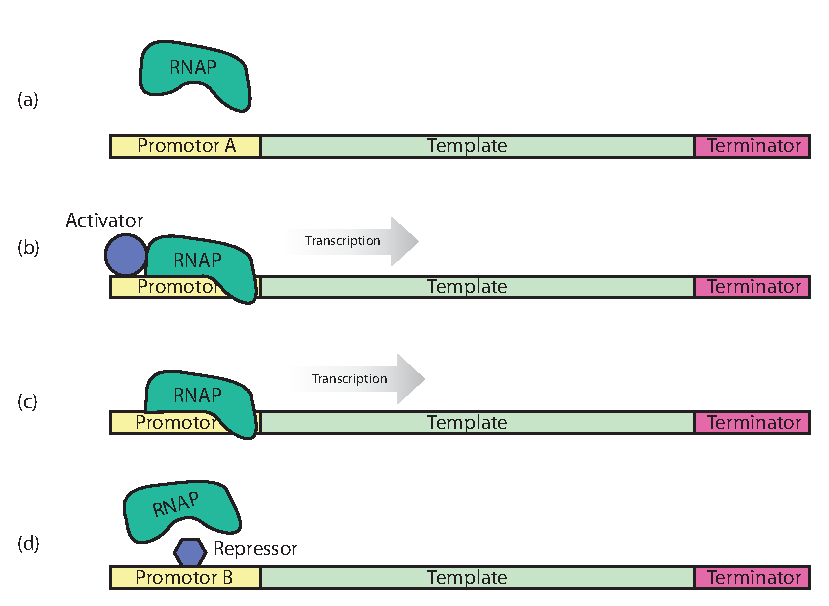
\epsfig{file=figures/regulation.eps, scale=0.75}
\caption{\label{fig:regulation}
  (a) RNAP has low affinity for promoter A. (b) The presence of a
  transcription factor specific to promoter A increases the affinity
  of RNAP for the promoter. (c) RNAP has high affinity for promoter
  B. The presence of a repressor specific to promoter B blocks RNAP
  from transcribing the gene.} 
\end{figure}

As shown in Figure~\ref{fig:regulation}, transcription factors can
either be {\em activators} or {\em repressors}. An activator $A$ works
by improving the affinity of RNAP for specific promoters $p_A$ that
are complimentary to $A$. In contrast, a repressor $R$ works by
blocking RNAP from docking to promoters of type $p_R$. For example,
the $LacI$ repressor (which is actually four identical proteins bound
together into a tetramer) is found in {\em E. coli}. It sticks very
selectively to the promoter $p_\mathit{lac}$ due to the three
dimensional structure of the DNA double helix comprising the
promoter. When bound, it prevents RNAP from binding to the
promoter. In general, promoters and transcription factors go together
and the sequence of $A$, $T$, $C$ and $G$ in the promoter determines a
three dimensional structure in the DNA helix that has some affinity
for RNAP and some affinity for some transcription factors (either zero
or more).

In addition to the above simple mechanisms, many transcription factors
work in groups so that transcription occurs as some function
%
$$
  \mathrm{rate\ of\ transcription}\ = \ f(T_1, ..., T_n) 
$$
%
of the concentrations of the transcription factors $T_1, ..., T_n$
associated with the gene. 

Many transcription factors take on active and inactive forms based on
the presence or absence of small molecules. Such transcription factors
thus form sensors. For example, the repressor $LacI$ is active when
there is none of the sugar lactose around. In its active form, $LacI$
represses the genes encoding the enzymes for incorporating and
metabolizing lactose. In the presence of lactose, the repressor
becomes inactive, and the lactose genes are transcribed (and
translated). In general, there are several ways in which a small
molecule can interact with a transcription factor -- these are
summarized in Figure~\ref{fig:trans-small}.

\begin{figure}
\centering
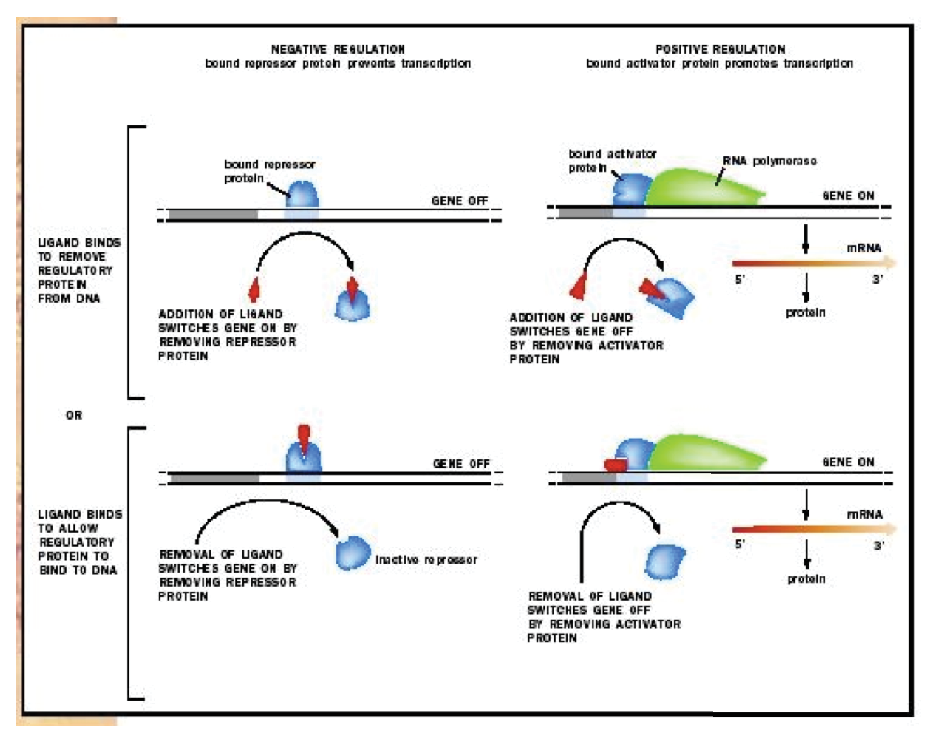
\epsfig{file=figures/trans-small.eps, scale=0.75}
\caption{\label{fig:trans-small}
  Small molecules can activate or deactivate transcription factors in
  a variety of ways. }
\end{figure}

Now consider a set of protein-coding genes $g_1, ..., g_n$. Draw each
gene as a circle. If a gene produces a transcription factor that
activates or represses another gene, we write an arrow or a line with
a bar respectively from one gene to the other. If a small molecule
activates or deactivates a transcription factor, we draw similar
arrows from nodes representing the molecule to the arrow representing
an interaction. The result is a {\em genetic regulator network}, and
example of which is shown in Figure~\ref{fig:grn}. 

\begin{figure}
\centering
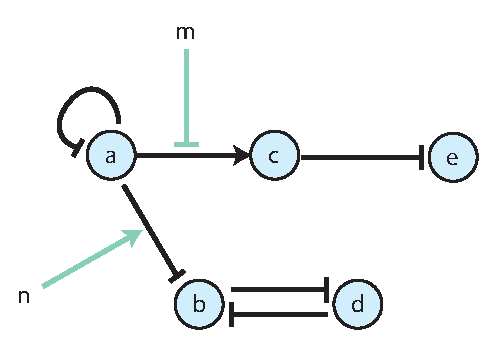
\epsfig{file=figures/grn.eps}
\caption{\label{fig:grn}
  Small molecules can activate or deactivate transcription factors in
  a variety of ways. }
\end{figure}

There are a host of other ways in which genes are regulated, not
always by proteins. For example, non-coding RNAs can interact with
mRNAs in a variety of ways, either preventing the mRNAs from being
transcribed, or even by allowing them to be transcribed. A good survey
of these mechanisms can be found in \cite{rna-synthetic-biology}.

\subsection{Metabolism}

A cell is a miniature chemical processing plant. Most cells can
synthesize a broad variety of substances from the raw materials they
take up from the environment. For example, {\em E. coli} can
synthesize, among other things, amino acids for protein construction,
nucleotides for RNA and DNA, and carbohydrates for energy
storage. Furthermore, the substances that cells take up are highly
variable, so many of the chemical reactions inside cells are designed
to break down nutrients into key energy carrying molecules (such as
ATP) and basic raw materials for later synthesis reactions (such as
pyruvate). Figure~\ref{fig:metabolism-overview} illustrates the
process of {\em catabolism} (breaking down nutrients) and {\em
  anabolism} (synthesizing) useful molecules. 

As described above, many proteins act as enzymes. An enzyme is a
catalyst that increases the backward and forward rate of a chemical
reaction (or family of reactions) by lowering the energy barrier
between the reactants and the products. By expressing some protein
enzymes and not others, the cell can steer metabolites through desired
pathways. Furthermore, by sensing metabolites (for example with
transcription factors that are activated by metabolites), a genetic
regulatory network can {\em control} the metabolism. 

\begin{figure}
\centering
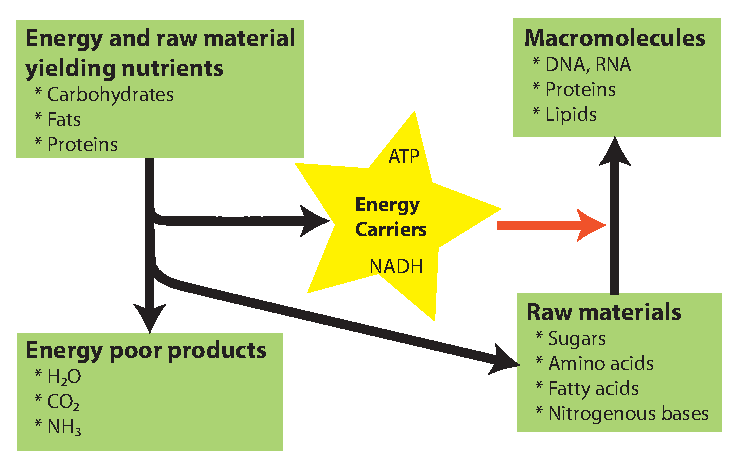
\epsfig{file=figures/metabolism-overview.eps, scale=0.7}
\caption{\label{fig:metabolism-overview}
  Metabolism ... }
\end{figure}

A complete description of all of the metabolic pathways in even {\em
  E. coli} is beyond the scope of this (and most other) texts. There are
an enormous number of metabolites and reactions. However, to give a
flavor of what is involved, we briefly describe a key metabolic
pathway that is fundamental to life, namely {\em
  glycolysis}. Glycolysis is found in every organism on the planet and
likely evolved very early.

The glycolytic pathway (glycolysis) essentially is responsible for
converting the sugar {\em glucose} into two molecules of {\em
  pyruvate} with a net gain in energy of two ATP molecules. Glucose is
a basic nutrient that can either be taken up by the cell from the
environment or obtained from carbohydrate energy storage. It has three
main destinies in the cell: (1) It can be put into storage; (2) it can
be used in the synthesis of small molecules such as nucleotides and
amino acids; (3) it's high-energy content can be used to make
ATP. The first step of the third destiny is glycolysis. Pyruvate, the
product of glycolysis, is still energetic and itself is a precursor
for several pathways, the most important of which is the citric acid
cycle, which milks the rest of the energy out of pyruvate by oxidizing
it.

The glycolysis pathway is shown in Figure~\ref{fig:glycolysis}. It
consists of a series of several steps. The names of the metabolites
are shown. Each one consists of a minor change to the metabolite
before it. In some steps ATP (adenosine triphosphate) is consumed to
produce ADP (adenosine diphosphate), which is an energy consuming
step. In other steps, ADP is consumed and ATP is produced. In the fifth
step, energy is also produced via the {\em cofactor} NAD$^+$. This
molecule is a cofactor of many steps in the metabolism of the cell
and, after ATP, is one of the most common players in metabolic
pathways. 

Each step in the pathway is labeled by the name of the enzyme
associated with the reaction. For example, the last step is catalyzed
by the enzyme {\em pyruvate kinase}, which increases the rate of the
reaction
%
$$
\mathrm{Phosphoenolpyruvate} + \mathrm{ADP}
  \leftrightharpoons \mathrm{Pyruvate} + \mathrm{ATP}.
$$
%
This step is essentially irreversible. We return to metabolism in
Chapter~\ref{ch:enzymes}. At that point, the analysis and control of
metabolic networks is discussed.

\begin{figure}
\centering
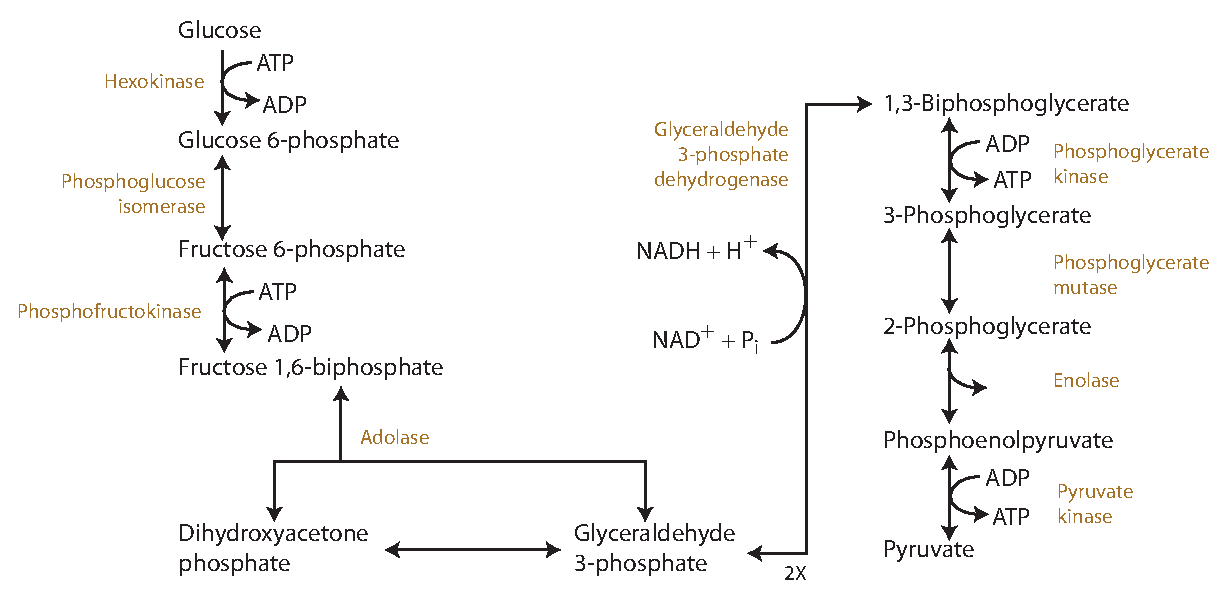
\epsfig{file=figures/glycolysis.eps, scale=0.6}
\caption{\label{fig:glycolysis}
  The glycolysis pathway. }
\end{figure}

Metabolic engineers have achieved astounding results by introducing
enzymes from one organism into others to rewrite their metabolic
pathways. For example, an enzyme from {\em Artemisia annua} (sweet
wormwood) that produces artemisinic acid was introduced into yeast
\cite{keasling-art}. Artemisinic acid is an expensive antimalarial
drug that, if it could be produced cheaply in yeast, could be very
useful in fighting malaria worldwide. However, presently it is still
not cost effective to produce this drug in yeast, mainly because
putting all of a yeast cell's resources into making artemisinic acid
makes the yeast cell unhealthy. Increasing the yields of the
artificial pathway over the past several years have involved
incredibly meticulous tuning of every step of the pathway starting
with Acetyl-CoA (one step after pyruvate) to artemisinic acid. It is
unclear how this tuning process can be automated, but if it could, the
synthesis of novel molecules in cells could become commonplace. 

\subsection{Signaling}

e.g. G-protein

\subsection{Growth and Division}

\section{Re-programming {\em E. coli}}

% how we program it (plasmids, etc)

A nice feature of {\em E. coli}, and other organisms as well, is that
an {\em E. coli} cell may contain one or more pieces of small,
circular {\em plasmid} DNA. These independently replicating pieces of
DNA are processed inside the cell much the same way as is genomic
DNA. Furthermore, it turns out to be fairly easy to construct
synthetic plasmids and stick them inside appropriately prepared
cells. Once there, the 

\section{How we See What's Going On}

% how we see what is going on: fluorescence, micrsoscopy, gene arrays,
% RT-pcr, flow-cytometry, etc. This can be brief. Perhaps a whole
% chapter can be devoted to it later.

% Regulation: Transcription factors, ribozymes and other mechanisms

% Observables: GFP, FRET, populations, single cells

% How to program cells

% Inputs: IPTG, UV, periodic inputs, etc.


\section{Problems}

\setcounter{exercount}{0}

\begin{exercise}
  An {\em E. coli} cell is an approximately 2 $\mu$m long cylinder with
  diameter 1 $\mu$m. What is its approximate volume? If there are
  about 3.6 million proteins inside a single cell, what is the
  concentration of protein in the cell in moles per liter?
\end{exercise}

\begin{exercise}
  The genetic code assigns an amino acid to each three letter sequence
  of nucleotides. How many genetic codes are possible? Why do you
  think all of the living systems (that we know of) use the same
  genetic code?
\end{exercise}

\begin{exercise}
  The molecular machinery for {\em copying} the DNA in a cell during
  cell-replication (not covered in this text) has very sophisticated
  error correction mechanisms. In contrast, the error correcting
  mechanisms for RNA polymerase (RNAP) are fairly limited -- and RNAP
  therefore makes more mistakes. Why should this be?
\end{exercise}

\begin{exercise}
  Find two different promoters in the BioBricks registry at
\begin{quote}
 \href{http://partsregistry.org/}{\tt http://partsregistry.org/}.
\end{quote}
Show the sequence of nucleotides in each and explain their
similarities and differences.
\end{exercise}

